%!TEX program = xelatex
\documentclass[a4paper, 12pt]{article}

\usepackage[no-math]{fontspec}
\usepackage[main = russian, english]{babel}
\usepackage{xunicode}
\usepackage{xltxtra}

\usepackage{amssymb}
\usepackage{mathtools}

\usepackage[sc]{mathpazo}
\usepackage[euler-digits,euler-hat-accent]{eulervm}

\usepackage{MnSymbol} % order is crucial


\defaultfontfeatures{Mapping=tex-text, Scale=MatchLowercase}
\setmainfont[
   BoldFont={Greta Text Pro Bold},
   ItalicFont={Greta Text Pro Italic},
   BoldItalicFont={Greta Text Pro Bold Italic}
]{Greta Text Pro Light}
\setmonofont[Mapping=tex-text]{Liberation Mono}
% \newfontfamily{\cyrillicfont}{TeX Gyre Pagella}
% \setromanfont{TeX Gyre Pagella}

% page props:
% \linespread{1.2}
\usepackage[top=0.5in, bottom=0.7in, left=0.6in, right=0.6in]{geometry}

\usepackage{parskip}
\usepackage{hyperref}
\usepackage{setspace}
\usepackage[shortlabels]{enumitem}

% ========= Graph stuff packages ==========
\usepackage{graphicx}
\usepackage{xcolor}
\usepackage{subfig}
\usepackage{tikz}
\usepackage{tkz-berge}

% ========= Special packages ==============
\usepackage{bussproofs}
\usepackage{stmaryrd}

% ========= Listings / algo packages =========
\usepackage{xifthen}
\usepackage{algorithm}
\usepackage[noend]{algpseudocode}
\usepackage{listings}

\lstdefinelanguage{GemlBeeLang}{
        language=Python,
        alsoletter={=,:},
        morekeywords={:=, where, then, AND, OR, NOT, WHERE, show, and, or, not, true, false, endif},
}

\definecolor{dkgreen}{rgb}{0,0.6,0}
\definecolor{mauve}{rgb}{0.5,0.37,0.37}

\lstset{
  frame=lrtb,
  language=GemlBeeLang,
  aboveskip=2mm,
  belowskip=2mm,
  showstringspaces=false,
  columns=fullflexible,
  basicstyle={\ttfamily},
  % numbers=left,
  numbers=none,
  numberstyle=\tiny\color{gray},
  keywordstyle=\color{blue},
  commentstyle=\color{dkgreen},
  stringstyle=\color{mauve},
  breaklines=true,
  breakatwhitespace=true,
  tabsize=4,
  backgroundcolor=\color{gray!7},
  showspaces=false,
  showtabs=false,
  escapeinside={(*@}{@*)},
  rulecolor=\color{gray!10}
}

\lstdefinestyle{nonumbers}{numbers=none}

\usetikzlibrary{shapes,snakes}
\usetikzlibrary{arrows, petri, topaths}
\linespread{1.3}
\setlist[enumerate, 1]{label = (\alph*)}


\newenvironment{task}[1][]
{
  \par\medskip
  \noindent \textbf{Задание~№#1}
  \rmfamily
}
{
}

\newenvironment{solution}[1][]
{
  \par
  \noindent \textbf{\textit{Решение:~}}
  \rmfamily
}
{
  \medskip
}

% Math and algorithms
\makeatletter
\renewcommand{\ALG@name}{Алгоритм}
\renewcommand{\listalgorithmname}{Список алгроитмов}
\newenvironment{procedure}[1]
  {\renewcommand*{\ALG@name}{Процедура}
  \algorithm\renewcommand{\thealgorithm}{\thechapter.\arabic{algorithm} #1}}
  {\endalgorithm}
\makeatother

\algrenewcommand\algorithmicrequire{\textbf{Вход:}}
\algrenewcommand\algorithmicensure{\textbf{Выход:}}
\algnewcommand\True{\textbf{true}\space}
\algnewcommand\False{\textbf{false}\space}
\algnewcommand\And{\textbf{and}\space}
\newcommand{\xfor}[3]{#1 \textbf{from} #2 \textbf{to} #3}
\newcommand{\xassign}[2]{\State #1 $\leftarrow$ #2}
\newcommand{\xstate}[1]{\State #1}
\newcommand{\xreturn}[1]{\xstate{\textbf{return} #1}}
\DeclarePairedDelimiter\ceil{\lceil}{\rceil}
\DeclarePairedDelimiter\floor{\lfloor}{\rfloor}
\newcommand{\bigO}[1]{\mathcal{O}\left(#1\right)}
\newcommand{\xqed}{\hfill $\blacksquare$}
\newcommand{\code}[1]{\colorbox{gray!15}{\footnotesize\texttt{#1}}}

% Commands (my)

\newcommand{\xparen}[1]{\left( #1 \right)}
\newcommand{\xangle}[1]{\left\langle #1 \right\rangle}
\newcommand{\xbracket}[1]{\left[ #1 \right]}
\newcommand{\xbrace}[1]{\left\lbrace #1 \right\rbrace}
\newcommand{\xret}[0]{\rightarrow}
\newcommand{\xintrp}[1]{\left\llbracket #1 \right\rrbracket}
\usepackage{tikz-qtree}
\usepackage{amsmath}
\usepackage{amsthm}
\usepackage{amsfonts}
\usepackage{hyperref}
\usepackage{booktabs}
\usepackage{tabu}
\usepackage{graphicx}
\usepackage{import}
\usepackage{mathtools}
\usepackage{hyphenat}
\usepackage{algorithm}
\usepackage[noend]{algpseudocode}

\usepackage{ulem}
\normalem

% algorithms
\makeatletter
\renewcommand{\ALG@name}{Алгоритм}
\renewcommand{\listalgorithmname}{Список алгроитмов}

\newenvironment{procedure}[1]
  {\renewcommand*{\ALG@name}{Процедура}
  \algorithm\renewcommand{\thealgorithm}{\thechapter.\arabic{algorithm} #1}}
  {\endalgorithm}

\makeatother

\algrenewcommand\algorithmicrequire{\textbf{Вход:}}
\algrenewcommand\algorithmicensure{\textbf{Выход:}}
\algnewcommand\True{\textbf{true}\space}
\algnewcommand\False{\textbf{false}\space}
\algnewcommand\And{\textbf{and}\space}


\newcommand{\algFor}[3]{#1 \textbf{from} #2 \textbf{to} #3}
\newcommand{\algAssign}[2]{\State #1 $\leftarrow$ #2}
\newcommand{\algState}[1]{\State #1}

\newcommand{\empht}[1]{\text{\emph{#1}}}
\newcommand{\trule}[2]{\text{#1} \rightarrow \text{#2}} % rule with text-labels (no italic stuff)

\newcommand{\inlineq}[1]{
	\hfill \makebox[0pt][r]{%
            \begin{minipage}[b]{\textwidth}
              \begin{equation}
                 #1
              \end{equation}
          \end{minipage}}
}

\usepackage[scale=2]{ccicons}

\usepgfplotslibrary{dateplot}


\title{SLAM в ROS}
\author{
Выполнил: \hfill студент Горбунов Е.А. \\
Руководитель: \hfill Кринкин К.В.
}
\institute{СПбАУ}

\begin{document}
\maketitle

\begin{frame}[fragile]{Предметная область}

\begin{figure}
\centering
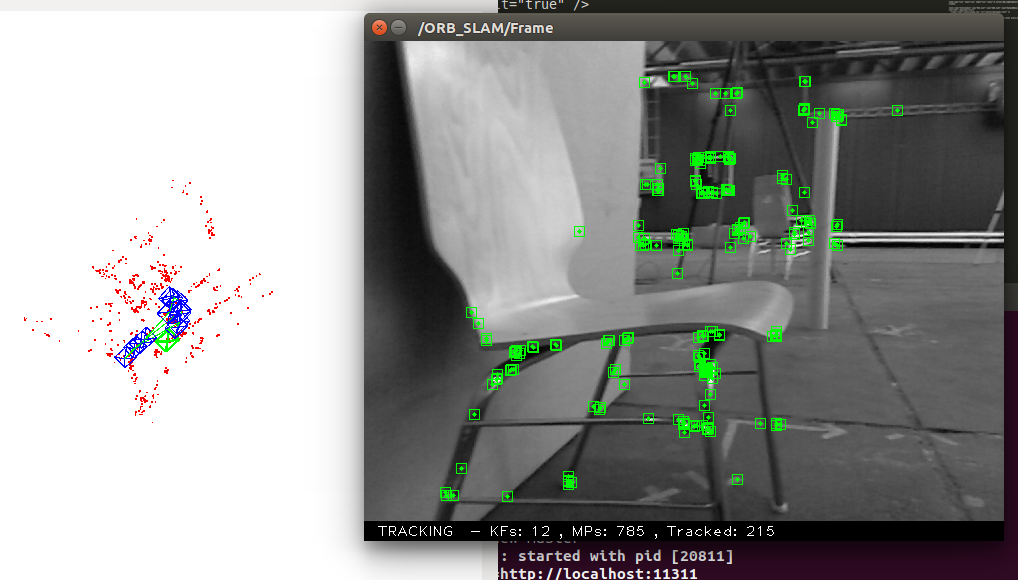
\includegraphics[scale=0.21]{data/slam_at_work_1}
\end{figure}
\begin{itemize}
\item Визуальный SLAM (Simultaneous Localization and Mapping)
\item Один из этапов алгоритма: извлечение особых точек (feature points detection)
\item ROS (Robotics operating system) --- фрэймворк для программирования роботов
\end{itemize}
\end{frame}

\begin{frame}{Постановка задачи}
\begin{enumerate}
\item Изучить наиболее популярные подходы к извлечению особых точек
\item Сделать утилиту, позволяющую извлекать и отображать особые точки на визуальных данных
	\begin{itemize}
		\item Поддержка загрузки картинок и видео
		\item Поддержка извлечения точек из проигрываемых bag-файлов (rosplay)
		\item Возможность менять параметры детекторов особых точек
	\end{itemize}
\item Провести сравнение изученных методов
\end{enumerate}
\end{frame}

\begin{frame}{Что тут уже сделали?}

\begin{itemize}
	\item Про особые точки и методы их извлечения написано много статей
	\item Поиски каких-то программ, чтобы на работу этих методов посмотреть не привели к результатам,
	к тому же с поддержкой bag-файлов
\end{itemize}

\end{frame}


\begin{frame}{Извлечение особых точек}
\begin{itemize}
	\item Особые точки --- точки с сильным изменением яркости в более чем 1 направлении (угловые точки)
	\item Характеристики:
	\begin{itemize}
		\item Устойчивость к масштабу, повороту
		\item Устойчивость к изменению освещения
		\item Сложность вычисления
	\end{itemize}
	\item Выбранные для изучения методы:
	\begin{itemize}
		\item SIFT (1999) --- классика
		\item SURF (2006) --- наследник SIFT
		\item FAST (2006)
		\item ORB (2011) --- используется в ORB-SLAM, использует FAST
	\end{itemize}
\end{itemize}
\end{frame}

\begin{frame}{Утилита для извлечения особых точек}
\begin{figure}
\centering
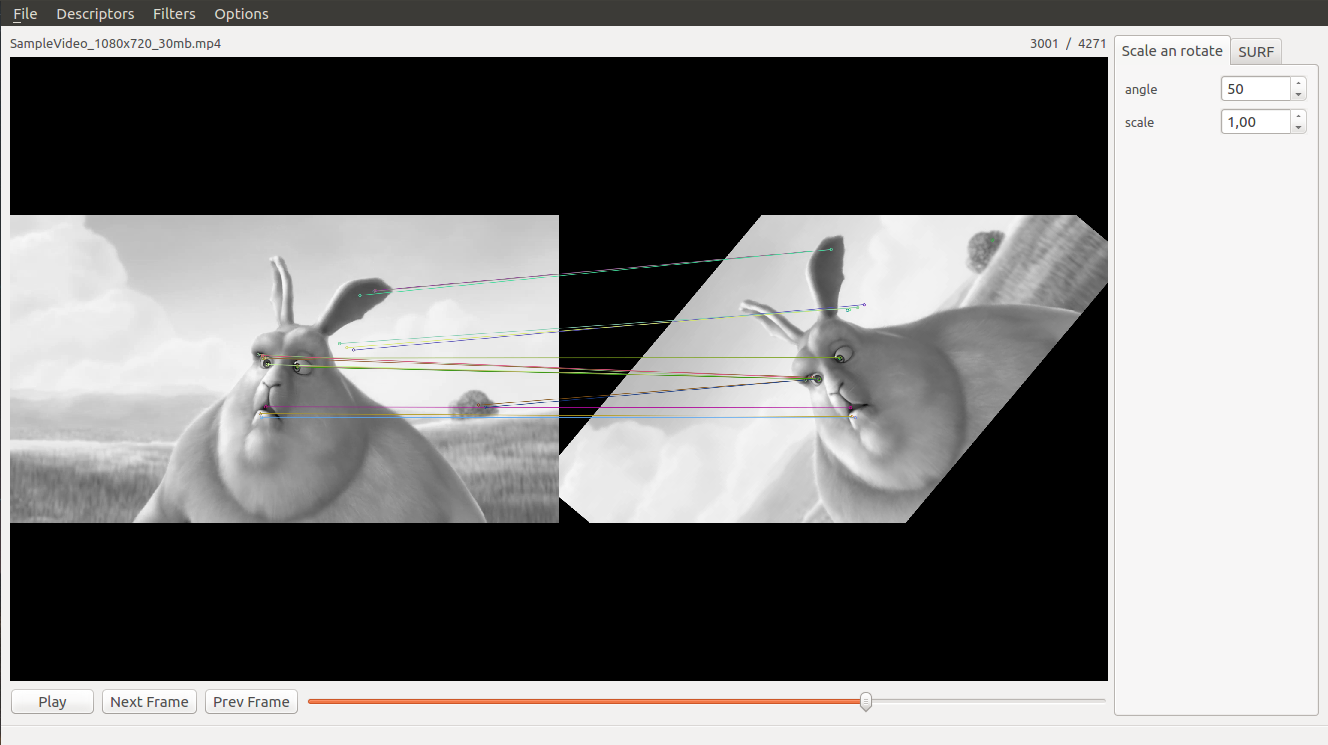
\includegraphics[scale=0.32]{data/Feature_match}
\end{figure}
\end{frame}

\begin{frame}{Что утилита может?}
\begin{itemize}
	\item Сопоставление особых точек на оригинальном кадре и кадре с наложенными фильтрами 
	\item Лёгкое добавление новых детекторов особых точек
	\item Лёгкое добавление фильтров с возможностью настройки их параметров
\end{itemize}
% \begin{figure}
% \centering
% 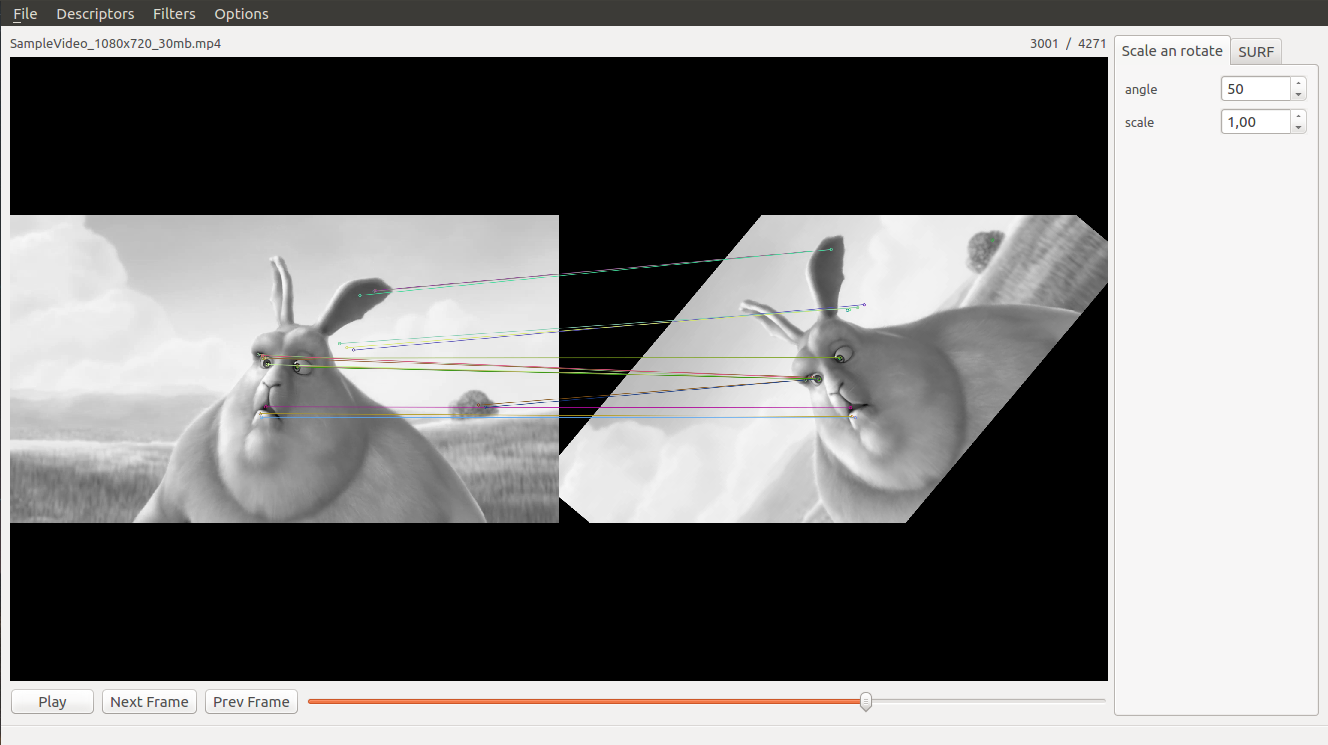
\includegraphics[scale=0.32]{data/Feature_match}
% \end{figure}
\end{frame}

\begin{frame}{Результаты}
\begin{enumerate}
	\item Страничка c описанием методов извлечения особых точек \url{dev.osll.ru/projects/robotics/wiki/Visual_Features_Taxonomy}
	\item Код утилиты для отображения особых точек в репозитории \url{dev.osll.ru/projects/robotics/repository} (robotics/utils/feature-detector)
\end{enumerate}
\end{frame}

\begin{frame}{Что нового узнал?}
\begin{itemize}
	\item Методы извлечения особых точек
	\item Работа с ROS (Robotics operating system)
	\item CMake + OpenCV + Qt
\end{itemize}
% Qt, ROS, Feature Detectors guts
\end{frame}

\plain{Конец}


\end{document}